\documentclass[9pt]{beamer}
\mode<presentation>

% Theme choice:
\usetheme{Madrid}%Darmstadt 

\usecolortheme[RGB={0,100,50}]{structure}
 \usefonttheme{structurebold} 
\setbeamercovered{invisible}
%\setbeamertemplate{navigation symbols}{}
\usepackage{dynblocks}
\usepackage{textpos}
\usepackage{amsfonts}
\usepackage{amsmath}
\usepackage{amssymb}
\usepackage{amsthm}

\newtheorem{teorema}{Teorema}\usepackage{mathtools}
\renewcommand{\proofname}{Prova}
\usepackage[portuguese]{babel}

\uselanguage{Portuguese}
\languagepath{Portuguese}

\deftranslation[to=Portuguese]{Theorem}{Teorema}
\deftranslation[to=Portuguese]{Lemma}{Lema}
\deftranslation[to=Portuguese]{Corollary}{Corolário}
\deftranslation[to=Portuguese]{Proof}{Prova}

\usepackage{dutchcal}
\usepackage{hyperref}
\usepackage[utf8]{inputenc}
\usepackage[T1]{fontenc}
\usepackage{amsthm}


\usepackage[affil-it]{authblk} 
\usepackage{etoolbox}
\usepackage{lmodern}

\makeatletter
\patchcmd{\@maketitle}{\LARGE \@title}{\fontsize{18}{19.2}\selectfont\@title}{}{}
\makeatother

\renewcommand\Authfont{\fontsize{12}{14.4}\selectfont}
\renewcommand\Affilfont{\fontsize{9}{10.8}\itshape}
 
% Title page details: 
\title[Presentation]{Lógica para Engenharia de Software} %add title


\institute[UniRV]{\textbf{\large  \textcolor{structure}{\textbf{\large
Proposições, Tabelas-Verdade, Implicação Lógica e Equivalência.
}} %add name 
% \hspace{0.5pt}
\\ \qquad
\\Professor: Me. Sergio Souza Novak 
\\Faculdade de Engenharia de Software}
} 
% \titlegraphic{\includegraphics[width=5cm]{msu.eps}}
\titlegraphic{
\includegraphics[width=5cm]{Universidade_de_Rio_Verde.jpg}}
\date{}

% Logo only on title page
%\logo{
\includegraphics[width=1cm,keepaspectratio]{Logo.png}}
\usepackage[pscoord]{eso-pic}


\begin{document}

% Title page frame
%\begin{frame}
    %\titlepage 
%\end{frame}
\frame[plain]{\titlepage}
%logo
\AddToShipoutPictureFG{
    \put(\LenToUnit{.92\paperwidth},
    \LenToUnit{.185\paperheight})
    {\vtop{{\null}
    \makebox{
\includegraphics[width=.8cm,keepaspectratio]{Universidade_de_Rio_Verde.jpg}}}}}


\begin{frame}{Sumário}
  \tableofcontents
\end{frame}
\section{Proposição lógica} 

\begin{frame}{Proposição}

\begin{block}{Definição}
Uma \textbf{proposição} é uma sentença declarativa à qual se pode atribuir
um valor lógico: \textbf{verdadeiro} ou \textbf{falso}, mas não ambos.
\end{block}

\begin{block}{Exemplos}
\begin{itemize}
    \item ``$2 + 2 = 4$'' (proposição verdadeira).
    \item ``$5$ é um número par'' (proposição falsa).
    \item ``Glifosato é um herbicida'' (proposição verdadeira).
\end{itemize}
\end{block}

\begin{block}{Não Exemplos}
As sentenças abaixo \textbf{não} são proposições:
\begin{itemize}
    \item ``Qual é a sua idade?'' (pergunta).
    \item ``Estude para a prova!'' (ordem).
\end{itemize}
\end{block}
 

\end{frame}

\section{Conjunção e disjunção}
\begin{frame}{Conectivos Lógicos: \textbf{E} ($\land$) e \textbf{OU} ($\lor$)}
\Large

\begin{block}{Definição}
\begin{itemize}
    \item \textbf{Conjunção} ($P \land Q$): verdadeira se \textbf{ambas} as proposições forem verdadeiras.
    \item \textbf{Disjunção} ($P \lor Q$): verdadeira se \textbf{ao menos uma} das proposições for verdadeira.
\end{itemize}
\end{block}

\begin{block}{Propriedades Fundamentais}
\begin{itemize}
    \item \textbf{Comutatividade}
    \[
        P \land Q \equiv Q \land P
        \qquad
        P \lor Q \equiv Q \lor P
    \]

    \item \textbf{Associatividade}
    \[
        (P \land Q) \land R \equiv P \land (Q \land R)
    \]
    \[
        (P \lor Q) \lor R \equiv P \lor (Q \lor R)
    \]

    \item \textbf{Idempotência}
    \[
        P \land P \equiv P
        \qquad
        P \lor P \equiv P
    \]
\end{itemize}
\end{block}

\end{frame}
 
\section{Tabela Verdade}
\begin{frame}{Tabelas-Verdade}
\begin{figure}[h]
    \centering
    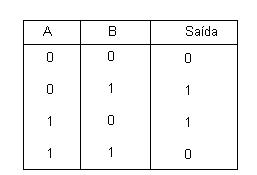
\includegraphics[width=0.4\linewidth]{tabela_verdade1.jpeg}
    \caption{exemplo de tabela-verdade.}
    \label{fig:meu_grafico}
\end{figure}
\begin{block}{Ideia Geral}
Um dos primeiros métodos propostos na literatura para a
verificação da validade de fórmulas da Lógica Proposicional
é o \textbf{método da tabela da verdade}.
\end{block}

\begin{block}{Definição}
A tabela da verdade é um método \textbf{exaustivo} de geração
de todas as valorações possíveis para uma dada fórmula lógica $A$.
\end{block}

\end{frame}
\begin{frame}{Construção da Tabela da Verdade}

\begin{block}{Estrutura da Tabela}
\begin{itemize}
    \item A tabela possui uma coluna para cada átomo e para cada saída.
    \item Os \textbf{átomos} aparecem nas colunas mais à esquerda.
    \item A fórmula principal aparece na coluna mais à direita.
\end{itemize}
\end{block}

\end{frame}

\begin{frame}{Exaustividade do Método}
\begin{figure}[h]
    \centering
    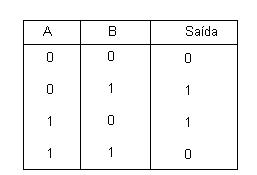
\includegraphics[width=0.4\linewidth]{tabela_verdade1.jpeg}
    \caption{exemplo de tabela-verdade.}
    \label{fig:meu_grafico}
\end{figure}
\begin{block}{Importante Observação}
Ao final da construção da tabela da verdade, \textbf{todas as possíveis
valorações da fórmula $A$ são consideradas}.
\end{block}

\begin{block}{Consequência}
Esse método garante correção lógica, porém pode ser computacionalmente
custoso.
\end{block}

\end{frame}
\begin{frame}{Complexidade Computacional}

\begin{block}{Número de Valorações}
Se uma fórmula contém $n$ átomos, então o número de valorações possíveis é:
\[
2^n
\]
\end{block}

\begin{block}{Número de Linhas}
Consequentemente, a tabela da verdade terá exatamente:
\[
2^n \text{ linhas}
\]
\end{block}

\end{frame}
\begin{frame}{Tabela-Verdade do Conectivo Negação}
\Large

\[
{\LARGE
\begin{array}{c|c}
p & \neg p \\ \hline
V & F \\
F & V
\end{array}
}
\]


\end{frame}

\begin{frame}{Tabela-Verdade do Conectivo E ($\land$)}
\LARGE
\[
\begin{array}{c|c|c}
    
p & q & p \land q \\ \hline
V & V & V \\
V & F & F \\
F & V & F \\
F & F & F
\end{array}
\]

\end{frame}
\begin{frame}{Tabela-Verdade do Conectivo OU ($\lor$)}
\LARGE
\[
\begin{array}{c|c|c}
p & q & p \lor q \\ \hline
V & V & V \\
V & F & V \\
F & V & V \\
F & F & F
\end{array}
\]

\end{frame}
\begin{frame}{Exemplo Completo de Tabela-Verdade}
\LARGE
\begin{block}{Fórmula}
\[
(P \lor Q) \land (\neg P \lor \neg Q)
\]
\end{block}

\[
\begin{array}{c|c|c|c|c|c|c}
P & Q & \neg P & \neg Q & P \lor Q & \neg P \lor \neg Q & (P \lor Q) \land (\neg P \lor \neg Q) \\ \hline
V & V & F & F & V & F & F \\
V & F & F & V & V & V & V \\
F & V & V & F & V & V & V \\
F & F & V & V & F & V & F
\end{array}
\]

\end{frame}
\section{Exercícios de Tabela Verdade}
\begin{frame}{Exercícios de Tabela-Verdade}
\Large

\begin{block}{Exercício 3 — Construção de Tabela}
Construa a tabela da verdade para a fórmula lógica:
\[
(P \land Q) \lor \neg Q
\]
\end{block}

\begin{block}{Orientação}
\begin{itemize}
    \item Liste todas as valorações possíveis de $P$ e $Q$;
    \item Avalie as subfórmulas;
    \item Determine o valor final da fórmula.
\end{itemize}
\end{block}

\end{frame}
\begin{frame}{Exercício Desafio}
\Large

\begin{block}{Exercício 4 — Análise da Fórmula}
Faça a tabela da verdade.
\[
(P \lor Q) \land (\neg P \land \neg Q)
\]
\end{block}

\begin{block}{Dica}
Observe se a fórmula assume valor verdadeiro:
\begin{itemize}
    \item em todas as linhas,
    \item em nenhuma linha,
    \item ou apenas em algumas linhas.
\end{itemize}
\end{block}

\end{frame}
\section{Hipótese}

\begin{frame}{Hipótese}

\begin{block}{Definição}
Em um contexto lógico ou matemático, uma \textbf{hipótese} é uma proposição
assumida como verdadeira para fins de análise, definição ou demonstração.
\end{block}

\begin{block}{Uso em Implicações}
Em uma implicação
\[
P \Rightarrow Q,
\]
a proposição $P$ é chamada de \textbf{hipótese},
enquanto $Q$ é chamada de \textbf{conclusão}.
\end{block}

\begin{block}{Exemplo}
Considere a afirmação:
\[
\text{``Se $x$ é par, então $x^2$ é par.''}
\]
Neste caso:
\begin{itemize}
    \item Hipótese: ``$x$ é par''.
    \item Conclusão: ``$x^2$ é par''.
\end{itemize}
\end{block}

\end{frame}
\begin{frame}{Tabelas-Verdade}

\begin{block}{O que é uma Tabela-Verdade}
Uma \textbf{tabela-verdade} é um instrumento lógico utilizado para determinar
o valor lógico de proposições compostas a partir dos valores lógicos
de suas proposições simples.
\end{block}

\begin{block}{Finalidade}
As tabelas-verdade permitem:
\begin{itemize}
    \item analisar conectivos lógicos (\(\neg, \land, \lor, \Rightarrow, \Leftrightarrow\));
    \item verificar se uma proposição é sempre verdadeira (tautologia);
    \item identificar contradições e contingências;
    \item comparar proposições quanto à equivalência lógica.
\end{itemize}
\end{block}

\begin{block}{Exemplo}
Considere a implicação \(P \Rightarrow Q\):
\[
\begin{array}{c|c|c}
P & Q & P \Rightarrow Q \\ \hline
V & V & V \\
V & F & F \\
F & V & V \\
F & F & V
\end{array}
\]
\end{block}

\end{frame}
\begin{frame}{Hipótese na Implicação Lógica}
\small

\begin{block}{Hipótese e Conclusão}
Em uma implicação lógica
\[
P \Rightarrow Q,
\]
a proposição $P$ é chamada de \textbf{hipótese}
e a proposição $Q$ é chamada de \textbf{conclusão}.
\end{block}

\begin{block}{Tabela-Verdade da Implicação}
\[
\begin{array}{c|c|c}
\text{Hipótese } (P) & \text{Conclusão } (Q) & P \Rightarrow Q \\ \hline
V & V & V \\
V & F & F \\
F & V & V \\
F & F & V
\end{array}
\]
\end{block}

\begin{block}{Interpretação}
\begin{itemize}
    \item Se $P$ é verdadeira e $Q$ é falsa, a implicação é falsa.
    \item Se $P$ é falsa, a implicação é verdadeira.
\end{itemize}
\end{block}

\end{frame}

\section{Implicação se P então Q}

\begin{frame}{Implicação Lógica — Contexto Histórico}

\begin{block}{Origens}
O conceito de implicação lógica tem origem na lógica aristotélica,
mas assume sua forma moderna a partir do século XIX com o desenvolvimento
da lógica simbólica.
\end{block}

\begin{block}{Evolução}
Matemáticos e lógicos como George Boole, Gottlob Frege e Bertrand Russell
formalizaram a implicação como um operador lógico fundamental,
permitindo a construção de sistemas dedutivos rigorosos.
\end{block}

\begin{block}{Importância}
A implicação lógica é a base das demonstrações matemáticas,
das definições formais e dos sistemas axiomáticos.
\end{block}

\end{frame}
\begin{frame}{Implicação Lógica — Intuição}

\begin{block}{Ideia Intuitiva}
A expressão
\[
P \Rightarrow Q
\]
deve ser lida como:
\begin{center}
\emph{``Se $P$ é verdadeiro, então $Q$ é verdadeiro.''}
\end{center}
\end{block}

\begin{block}{Relação de Dependência}
A implicação estabelece uma relação de dependência lógica entre proposições,
não uma relação de causalidade.
\end{block}

\begin{block}{Exemplo Simples}
Se um número é múltiplo de $4$, então é par:
\[
x \text{ é múltiplo de } 4 \Rightarrow x \text{ é par}.
\]
\end{block}

\end{frame}
\begin{frame}{Implicação Lógica — Definição Formal}

\begin{block}{Definição}
Sejam $P$ e $Q$ proposições.
Define-se a implicação lógica
\[
P \Rightarrow Q
\]
como a proposição que é falsa apenas quando $P$ é verdadeira
e $Q$ é falsa.
\end{block}

\begin{block}{Caracterização}
Em todos os demais casos, a implicação $P \Rightarrow Q$ é verdadeira.
\end{block}

\begin{block}{Observação}
Essa definição permite tratar a implicação de forma puramente lógica,
independente de interpretação semântica.
\end{block}

\end{frame}
\begin{frame}{Implicação Lógica e Quantificadores}

\begin{block}{Uso em Definições}
A implicação lógica aparece naturalmente em definições matemáticas,
como na definição de subconjunto:
\[
A \subseteq B \;\Longleftrightarrow\;
\forall x,\; (x \in A \Rightarrow x \in B).
\]
\end{block}

\begin{block}{Interpretação}
A implicação restringe o comportamento dos elementos que satisfazem
a condição inicial.
\end{block}

\begin{block}{Importância}
Sem a implicação, não seria possível formalizar corretamente conceitos
como inclusão, função e continuidade.
\end{block}

\end{frame}
\begin{frame}{Implicação Lógica — Propriedades}

\begin{block}{Propriedade Fundamental}
Se $P$ é falsa, então a implicação
\[
P \Rightarrow Q
\]
é verdadeira para qualquer proposição $Q$.
\end{block}

\begin{block}{Bicondicional}
Quando $P \Rightarrow Q$ e $Q \Rightarrow P$ são verdadeiras,
escreve-se
\[
P \Leftrightarrow Q,
\]
denominado \textbf{bicondicional}.
\end{block}

\begin{block}{Conclusão}
A implicação lógica é um dos operadores centrais da lógica matemática
e sustenta a estrutura das demonstrações formais.
\end{block}

\end{frame}
\section{Volta da implicação lógica}

\begin{frame}{Volta da Implicação Lógica}
\small

\begin{block}{Implicação Direta}
Uma implicação lógica é uma proposição da forma
\[
P \Rightarrow Q,
\]
lida como “se $P$, então $Q$”.
\end{block}

\begin{block}{Volta (Conversa) da Implicação}
A \textbf{volta da implicação} consiste em inverter
hipótese e conclusão, obtendo:
\[
Q \Rightarrow P.
\]
\end{block}

\begin{block}{Observação}
Em geral,
\[
P \Rightarrow Q \;\;\not\Rightarrow\;\; Q \Rightarrow P.
\]
Ou seja, a implicação não é reversível.
\end{block}

\end{frame}
\begin{frame}{Exemplos da Volta da Implicação}
\small

\begin{block}{Exemplo 1}
\begin{itemize}
    \item Implicação:  
    Se um número é múltiplo de 4, então é par.
    \[
    P \Rightarrow Q
    \]
    \item Volta:  
    Se um número é par, então é múltiplo de 4. \quad (Falsa)
\end{itemize}
\end{block}

\begin{block}{Exemplo 2}
\begin{itemize}
    \item Implicação:  
    Se um número é igual a 2, então é primo.
    \item Volta:  
    Se um número é primo, então é igual a 2. \quad (Falsa)
\end{itemize}
\end{block}

\begin{block}{Conclusão}
A verdade da implicação direta
não garante a verdade de sua volta.
\end{block}

\end{frame}
\section{Tabela Verdade como Método de Prova}

\begin{frame}{Tabelas-Verdade como Método de Prova}
\small

\begin{block}{Objetivo}
As tabelas-verdade permitem verificar a validade lógica
de proposições analisando \textbf{todos os valores possíveis}
das proposições envolvidas.
\end{block}

\begin{block}{Aplicações}
\begin{itemize}
    \item Verificar se uma implicação é válida
    \item Analisar o papel da hipótese
    \item Provar equivalência lógica entre proposições
\end{itemize}
\end{block}

\end{frame}
\begin{frame}{Hipótese na Implicação Lógica}
\small

\begin{block}{Definição}
Uma implicação lógica é uma proposição da forma
\[
P \Rightarrow Q,
\]
onde $P$ é a \textbf{hipótese} e $Q$ é a \textbf{conclusão}.
\end{block}

\begin{block}{Tabela-Verdade}
\[
\begin{array}{c|c|c}
P & Q & P \Rightarrow Q \\ \hline
V & V & V \\
V & F & F \\
F & V & V \\
F & F & V
\end{array}
\]
\end{block}

\end{frame}
\begin{frame}{Análise Formal da Hipótese pela Tabela-Verdade}
\small

\begin{block}{Caracterização Lógica da Implicação}
Para quaisquer proposições $P$ e $Q$, vale que
\[
P \Rightarrow Q \text{ é falsa}
\;\;\Longleftrightarrow\;\;
(P = V) \land (Q = F).
\]
Equivalentemente,
\[
\forall P\,\forall Q,\;
(P \Rightarrow Q = F)
\iff
(P = V \land Q = F).
\]
\end{block}

\begin{block}{Consequência Formal}
\[
\forall P\,\forall Q,\;
(P = F) \;\Rightarrow\; (P \Rightarrow Q = V).
\]
Ou seja, quando a hipótese é falsa,
a implicação é verdadeira, independentemente de $Q$.
\end{block}

\begin{block}{Conclusão}
A validade de $P \Rightarrow Q$ depende exclusivamente
das valorações em que a hipótese $P$ é verdadeira.
\end{block}

\end{frame}
\section{Exercícios de Implicação e Bicondicional}

% =======================
% Slide 1: Bicondicional
% =======================
\begin{frame}{Bicondicional: $S \Leftrightarrow X$}
\Large

\begin{block}{Definição}
A proposição $S \Leftrightarrow X$ é verdadeira quando $S$ e $X$ têm o mesmo valor lógico (ambas verdadeiras ou ambas falsas).
\end{block}

\begin{block}{Tabela-Verdade}
\[
\begin{array}{c|c|c}
S & X & S \Leftrightarrow X \\ \hline
V & V & V \\
V & F & F \\
F & V & F \\
F & F & V
\end{array}
\]
\end{block}

\begin{block}{Interpretação}
O bicondicional só falha quando os valores de $S$ e $X$ são diferentes.
\end{block}

\end{frame}





% \section{Definição de conjuntos e representação }
% \begin{frame}{Definição Formal de Conjuntos}

% \begin{block}{Conjunto}
% Um \textbf{conjunto} é uma coleção bem definida de elementos distintos, denominada por uma letra maiúscula, cujos elementos pertencem a um universo de discurso.
% \end{block}

% Seja $A$ um conjunto e $x$ um elemento qualquer. Dizemos que:
% \[
% x \in A \quad \text{se } x \text{ pertence a } A,
% \]
% \[
% x \notin A \quad \text{se } x \text{ não pertence a } A.
% \]

% \begin{block}{Definição por Extensão}
% Um conjunto pode ser definido listando explicitamente seus elementos:
% \[
% A = \{a_1, a_2, \dots, a_n\}.
% \]
% \end{block}

% \begin{block}{Definição por Compreensão}
% Um conjunto também pode ser definido por uma propriedade:
% \[
% A = \{\, x \in U \mid P(x) \,\},
% \]
% onde $U$ é o universo e $P(x)$ é uma proposição lógica.
% \end{block}

% \end{frame}
% \begin{frame}{Conjuntos Definidos por Extensão}

% \begin{block}{Definição por Extensão}
% Um conjunto é definido por \textbf{extensão} quando seus elementos são explicitamente enumerados.
% \end{block}

% \begin{block}{Conjunto dos Números Pares (Extensão)}
% O conjunto dos números pares pode ser definido como:
% \[
% P = \{0, 2, 4, 6, 8, \dots\}.
% \]
% \end{block}

% \begin{block}{Observação}
% A definição por extensão é adequada quando o conjunto é finito ou quando seus elementos seguem um padrão facilmente reconhecível.
% \end{block}

% \end{frame}
% \begin{frame}{Conjuntos Definidos por Compreensão}

% \begin{block}{Definição por Compreensão}
% Um conjunto é definido por \textbf{compreensão} quando seus elementos são caracterizados por uma propriedade lógica.
% \end{block}

% \begin{block}{Conjunto dos Números Pares (Compreensão)}
% O conjunto dos números pares pode ser definido como:
% \[
% P = \{\, x \in \mathbb{Z} \mid \exists k \in \mathbb{Z},\ x = 2k \,\}.
% \]
% \end{block}

% \begin{block}{Observação}
% A definição por compreensão permite descrever conjuntos infinitos de forma precisa e formal.
% \end{block}

% \end{frame}
% \section{Conjunto Vazio}

% \begin{frame}{Conjunto Vazio}
% \begin{figure}[h]
%     \centering
%     
\includegraphics[width=0.1\linewidth]{conjunto_vazio.png}
%     \caption{Conjunto vazio representado por um círculo sem elementos.}
%     \label{fig:meu_grafico}
% \end{figure}
% \begin{block}{Definição}
% O \textbf{conjunto vazio}, denotado por $\varnothing$ ou $\emptyset$, é o conjunto que não possui nenhum elemento.
% \end{block}

% \begin{block}{Caracterização Formal}
% Um conjunto $A$ é vazio se, e somente se,
% \[
% \forall x,\; x \notin A.
% \] 
% \end{block} 

% \begin{block}{Observação}
% O conjunto vazio é único e é subconjunto de qualquer conjunto.
% \end{block}

% \end{frame}
% \begin{frame}{Conjunto Vazio}

% \begin{block}{Caracterização Formal}
% Define-se o conjunto vazio, denotado por $\varnothing$, como o conjunto tal que
% \[
% \forall x,\; \bigl( x \in \varnothing \iff x \neq x \bigr).
% \]
% Equivalentemente,
% \[
% \varnothing = \{\, x \mid x \neq x \,\}.
% \]
% \end{block}

% \begin{block}{Justificativa}
% Como a proposição lógica $x \neq x$ é falsa para todo $x$, segue que
% \[
% \forall x,\; x \notin \varnothing.
% \]
% Logo, o conjunto $\varnothing$ não possui elementos.
% \end{block}

% \begin{block}{Observação}
% O conjunto vazio é único e é subconjunto de qualquer conjunto, isto é,
% \[
% \forall A,\; \varnothing \subseteq A.
% \]
% \end{block}

% \end{frame}


% \begin{frame}{Exemplos de Conjunto Vazio}

% \begin{block}{Exemplos}
% Cada um dos conjuntos a seguir é vazio, pois nenhuma condição apresentada pode ser satisfeita:
% \[
% \begin{aligned}
% A_1 &= \{\, x \in \mathbb{R} \mid x \neq x \,\} \\[4pt]
% A_2 &= \{\, (x,y) \in \mathbb{R}^2 \mid 
% \begin{cases}
% x + y = 1 \\
% x + y = 2
% \end{cases} \,\} \\[6pt]
% A_3 &= \{\, x \in \mathbb{N} \mid x < 0 \,\} \\[4pt]
% A_4 &= \{\, x \in \mathbb{R} \mid x^2 < 0 \,\} \\[4pt]
% \end{aligned}
% \]
% \end{block}

% \end{frame} 
 
% \begin{frame}{Exemplos de Conjunto Vazio}

% \begin{block}{Exemplos}
% Cada um dos conjuntos a seguir é vazio, pois nenhuma condição apresentada pode ser satisfeita:
% \[
% A_5 = \{\, x \in \mathbb{Z} \mid (\exists k \in \mathbb{Z},\ x = 2k)\ \land\ (\exists \ell \in \mathbb{Z},\ x = 2\ell + 1) \,\}
% \]
% \end{block}

% \end{frame}
% \begin{frame}{Cardinalidade de Conjuntos}

% \begin{block}{Definição}
% Seja $A$ um conjunto. Chama-se \textbf{cardinalidade} de $A$,
% denotada por $|A|$, o número de elementos de $A$.
% \end{block}

% \begin{block}{Caracterização Formal}
% Um conjunto $A$ é dito \textbf{finito} se existe um número natural $n \in \mathbb{N}$
% tal que $A$ possui exatamente $n$ elementos.
% Nesse caso, escreve-se
% \[
% |A| = n.
% \]
% \end{block}

% \begin{block}{Observação}
% Se não existe tal número natural, o conjunto é dito \textbf{infinito}.
% \end{block}

% \end{frame}
% \begin{frame}{Exemplo de Conjunto Finito}

% \begin{block}{Exemplo}
% Considere o conjunto
% \[
% A = \{1, 3, 5, 7\}.
% \]
% \end{block}

% \begin{block}{Análise}
% O conjunto $A$ possui exatamente quatro elementos.
% Logo, sua cardinalidade é
% \[
% |A| = 4.
% \]
% \end{block}

% \begin{block}{Conclusão}
% O conjunto $A$ é um conjunto finito.
% \end{block}

% \end{frame}
%     \begin{frame}{Exemplo de Conjunto Infinito}

% \begin{block}{Exemplo}
% Considere o conjunto dos números naturais
% \[
% \mathbb{N} = \{0, 1, 2, 3, 4, \dots\}.
% \]
% \end{block}

% \begin{block}{Análise}
% Para qualquer número natural $n$, existe sempre um sucessor $n+1 \in \mathbb{N}$.
% Assim, não é possível enumerar todos os seus elementos com um número finito.
% \end{block}

% \begin{block}{Conclusão}
% O conjunto $\mathbb{N}$ é infinito.
% \end{block}

% \end{frame}
% \begin{frame}{O Símbolo Seta}

% \begin{block}{Motivação}
% Em lógica e matemática, o símbolo seta é amplamente utilizado para expressar
% \textbf{relações de dependência lógica} entre proposições.
% \end{block}

% \begin{block}{Ideia Intuitiva}
% A expressão
% \[
% P \Rightarrow Q
% \]
% lê-se:
% \begin{center}
% \emph{``Se $P$ é verdadeiro, então $Q$ é verdadeiro.''}
% \end{center}
% \end{block}

% \begin{block}{Uso em Matemática}
% O símbolo $\Rightarrow$ aparece frequentemente em definições,
% demonstrações e caracterizações formais.
% \end{block}

% \end{frame}
% \begin{frame}{Definição Formal da Implicação}

% \begin{block}{Definição}
% Sejam $P$ e $Q$ proposições.
% A implicação
% \[
% P \Rightarrow Q
% \]
% é verdadeira sempre que a veracidade de $P$ implica a veracidade de $Q$.
% \end{block}

% \begin{block}{Caracterização Lógica}
% A implicação $P \Rightarrow Q$ é falsa \textbf{somente} no caso em que
% $P$ é verdadeira e $Q$ é falsa.
% \end{block}

% \begin{block}{Observação}
% Se $P$ é falsa, a implicação $P \Rightarrow Q$ é considerada verdadeira,
% independentemente do valor lógico de $Q$.
% \end{block}

% \end{frame}
% \begin{frame}{Exemplos de Implicação}

% \begin{block}{Exemplo 1 — Aritmética}
% Se $x$ é um número par, então $x^2$ é par:
% \[
% x \text{ é par } \Rightarrow x^2 \text{ é par}.
% \]
% \end{block}

% \begin{block}{Exemplo 2 — Conjuntos}
% Se um elemento pertence ao conjunto $A$ e $A \subseteq B$, então ele pertence a $B$:
% \[
% x \in A \Rightarrow x \in B.
% \]
% \end{block}

% \begin{block}{Exemplo 3 — Definições}
% A definição de subconjunto utiliza diretamente a implicação lógica:
% \[
% A \subseteq B \Rightarrow \forall x,\; (x \in A \Rightarrow x \in B).
% \]
% \end{block}

% \end{frame}
% \begin{frame}{Erros Comuns com o Símbolo Seta}

% \begin{block}{Erro 1 — Confundir com Bicondicional}
% A implicação
% \[
% P \Rightarrow Q
% \]
% não significa que $Q \Rightarrow P$ seja verdadeiro.
% \end{block}

% \begin{block}{Erro 2 — Confundir com Igualdade}
% A expressão
% \[
% P \Rightarrow Q
% \]
% não significa que $P$ e $Q$ sejam equivalentes.
% \end{block}

% \begin{block}{Observação Final}
% Quando ambos os sentidos são verdadeiros, utiliza-se o símbolo
% \[
% P \Leftrightarrow Q
% \]
% denominado \textbf{bicondicional}.
% \end{block}

% \end{frame}

% \begin{frame}{Pertinência}
% \begin{figure}[h]
%     \centering
%     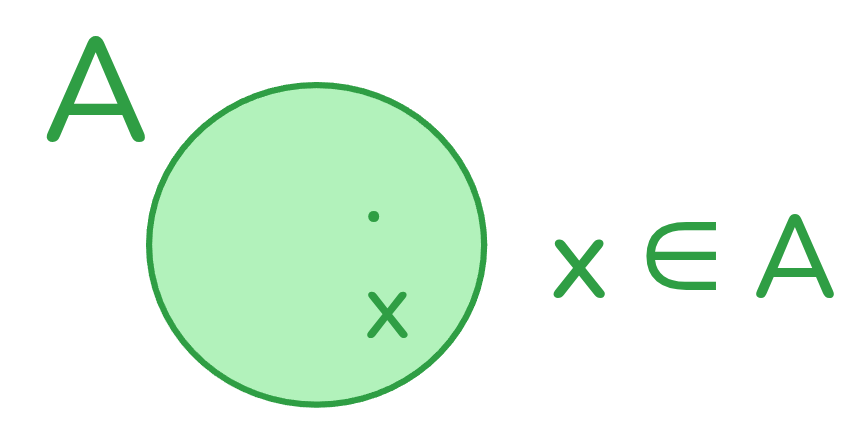
\includegraphics[width=0.6\linewidth]{pertence.png}
%     \caption{Conjunto vazio representado por um círculo sem elementos.}
%     \label{fig:meu_grafico}
% \end{figure}
% \begin{block}{Pertinência}
% Seja $A$ um conjunto e $x$ um elemento.
% Diz-se que $x$ \textbf{pertence} a $A$ se $x$ é um elemento de $A$,
% o que se denota por
% \[
% x \in A.
% \]
% Caso contrário, escreve-se
% \[
% x \notin A.
% \]
% \end{block}

% \end{frame}

% \begin{frame}{Continência}

% \begin{figure}[h]
%     \centering
%     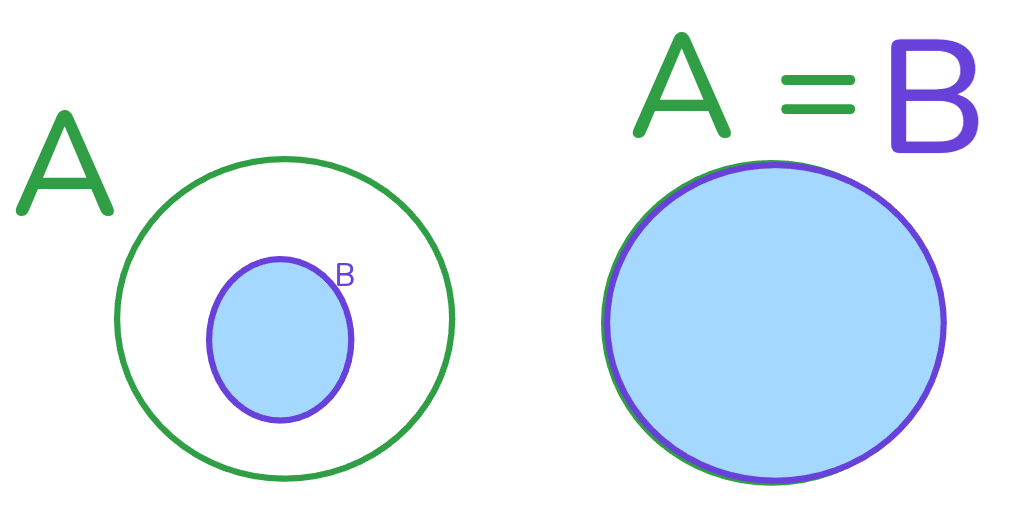
\includegraphics[width=0.6\linewidth]{contido.png}
%     \caption{Conjunto A contém B representado por um círculo maior (A) contendo um círculo menor (B).}
%     \label{fig:meu_grafico}
% \end{figure}

% \begin{block}{Continência}
% Sejam $A$ e $B$ conjuntos.
% Diz-se que $A$ está \textbf{contido} em $B$, ou que $A$ é subconjunto de $B$, se,
% por definição,
% \[
% A \subseteq B \;\stackrel{\text{def}}{\Longleftrightarrow}\;
% \forall x,\; (x \in A \Rightarrow x \in B).
% \]
% \end{block}
% \end{frame}

% \begin{frame}{Pertinência e Continência}

% \begin{block}{Pertinência}
% Seja $A$ um conjunto e $x$ um elemento.
% Diz-se que $x$ \textbf{pertence} a $A$ se $x$ é um elemento de $A$,
% o que se denota por
% \[
% x \in A.
% \]
% Caso contrário, escreve-se
% \[
% x \notin A.
% \]
% \end{block}

% \begin{block}{Continência}
% Sejam $A$ e $B$ conjuntos.
% Diz-se que $A$ está \textbf{contido} em $B$, ou que $A$ é subconjunto de $B$, se,
% por definição,
% \[
% A \subseteq B \;\stackrel{\text{def}}{\Longleftrightarrow}\;
% \forall x,\; (x \in A \Rightarrow x \in B).
% \]
% \end{block}

% \begin{block}{Observação Importante}
% A pertinência relaciona \textbf{elemento–conjunto}, enquanto a continência relaciona
% \textbf{conjunto–conjunto}.
% Assim, $x \in A$ e $A \subseteq B$ são relações de naturezas distintas.
% \end{block}

% \end{frame}



 


\end{document}
